\chapter{\;\;\;\;Formal Semantics}
\label{sec:main-semantics}

%% ``\#'' 은 넣을지 말지 애매한 것들입니다.

%% \begin{enumerate}
%% \item Interaction semantics
  %% \begin{enumerate}
    %% \item genv 초기화
    %% \item state, step/call/return
    %% \item system call module (?)
  %% \end{enumerate}
%% \item C wrapper semantics
%%   \begin{enumerate}
%%   \item \cc{} 대충 설명
%%   \item typify (\ccc{}와 비교)
%%   \end{enumerate}
%% \youngju{typify will be explained later when we explain upper bound}
%% \item Asm semantics
%%   \begin{enumerate}
  %% \item \cc{} 대충 설명
  %% \item junk pointer와 callee-save checking
  %% \item memory permission (\ccc{}와 비교) \\
  %%    unfree temporarily breaks axiom but it is ok
  %% \item (\#) PC만 보고 call/step/return 구분하는 법 (\ccc{}와 비교)
%%   \end{enumerate}
%% \end{enumerate}

%% \todo{dummy stack?}

%% \youngju{\ccc{}는 메모리, state 분리해서 after external 같은게 메모리 안받는데 우리는 \cc{}와의 차이를 줄이기 위해 분리 안했다는 이야기 언급}



%% \begin{figure}
%%   \centering
%%   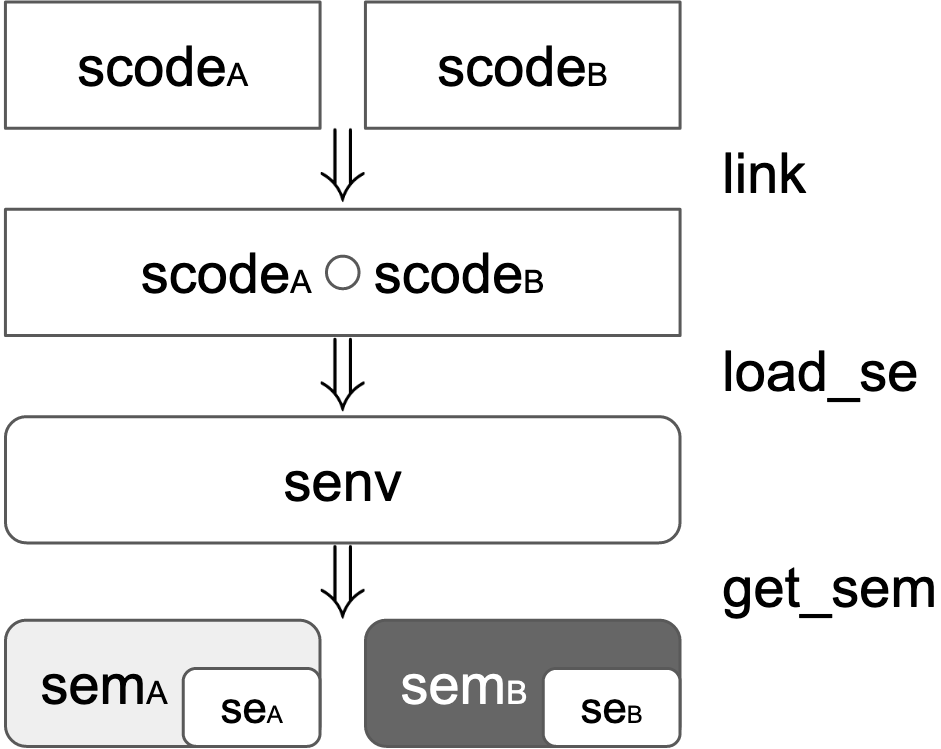
\includegraphics[width=0.25\linewidth]{fig-load.png}
%%   \caption{Loading Process}
%%   \label{fig:load}
%% \end{figure}


In this section we give a few interesting details of formal semantics: the loading of interaction
semantics (\Cref{sec:main-semantics:loading}) and a few tweaks we made for module semantics
(\Cref{sec:main-semantics:module}).


\section{Loading in Interaction Semantics}
\label{sec:main-semantics:loading}

\begin{wrapfigure}{R}{0.37\linewidth}
%% \small
%% \begin{minipage}[t]{0.65\linewidth}
%%   \mytitle{interaction semantics}\\
%% $
%%   %% \begin{stackTL}
%%   %%   state \triangleq (\Memory, \overrightarrow{(\msem, \msem.\texttt{state})}) \\
%%   %%   (\istt, \mem) \iestep{e} (\istt', \mem') \defeq \\
%%   %%   \begin{array}{l@{\;}l@{\;}l}
%%   %%     & \caselabel{STEP} & \forall \msem, \tl, e, \mem, \stt, \mem', \stt',~ (\mem, \stt) \estep{e} (\mem', \stt') \implies (\mem, ((\msem, \stt) \cons \tl)) \iestep{e} (\mem', (\msem, \stt') \cons \tl) \\
%%   %%     & \caselabel{CALL} & \forall \msem, \msem', \tl, \mem, \mem', \stt_{\msem}, \args, \stt_{\msem'},~
%%   %%       \msem.\texttt{at\_external} \; (\mem, \stt) \; \args \land \msem'.\texttt{init\_core} \; \args \; (\mem', \stt') \implies \\
%%   %%     & & (\mem, (\msem, \stt) \cons \tl) \iestep{e} (\mem', (\msem', \stt') \cons (\msem, \stt) \cons \tl) \\
%%   %%     & \caselabel{RET} & \forall \msem, \msem', \tl, \mem, \mem', \stt_{\msem}, \args, \stt_{\msem'},~
%%   %%       \msem.\texttt{halted} \; (\mem, \stt) \; \retv \land \msem'.\texttt{after\_external} \; \stt' \; \retv \; (\mem', \stt'') \implies \\
%%   %%     & & (\mem, (\msem, \stt) \cons (\msem', \stt') \cons \tl) \iestep{e} (\mem', (\msem', \stt'') \cons \tl) \\
%%   %%   \end{array}
%%   %% \end{stackTL}
%%   \begin{stackTL}
%%     %% \textrm{State} \defeq (\Memory, \overrightarrow{(\msem, \States{\msem})}) \\
%%     %% \textrm{State} \defeq \Memory \times \overrightarrow{\Msem \times \States{\Msem}} \\
%%     \textrm{State} \defeq \{ (\mem, \overrightarrow{(\msem, \stt)} \; | \; \mem \in \Memory \land \msem \in \Msem \land \stt \in \msem.\texttt{state} \} \\
%%     \Genv \defeq \{ \genv \; | \; \genv \in \overrightarrow{\Msem} \} \\
%%     \genv.\texttt{lookup\_modsem}(f) \defeq \{ \msem \; | \; \msem \in \genv \land f \in \textrm{ftns}(\msem.\texttt{senv}) \} \\
%%     \begin{array}{l@{\;}l@{\;}l}
%%       & \caselabel{STEP} & \genv \models (\mem, ((\msem, \stt) \cons \tl)) \iestep{e} (\mem', (\msem, \stt') \cons \tl) \myif \\
%%       & & (\mem, \stt) \estep{e} (\mem', \stt') \\
%%       & \caselabel{CALL} & \genv \models (\mem, (\msem, \stt) \cons \tl) \iestep{e} (\mem', (\msem', \stt') \cons (\msem, \stt) \cons \tl) \myif \\
%%       & & \exists \args,~ \msem.\texttt{at\_external}(\mem, \stt) = \some{\args} \land \msem' \in \genv.\texttt{lookup\_modsem}(c.\texttt{f}) \; \land \\
%%       & & (\mem', \stt') \in \msem'.\texttt{init\_core}(\args) \\
%%       & \caselabel{RET}  & \genv \models (\mem, (\msem, \stt) \cons (\msem', \stt') \cons \tl) \iestep{e} (\mem', (\msem', \stt'') \cons \tl) \myif \\
%%       & & \exists \retv,~ \msem.\texttt{halted}(\mem, \stt) = \some{\retv} \; \land \\
%%       & & \msem'.\texttt{after\_external}(\stt',\retv) = \some{(\mem', \stt'')} \\
%%     \end{array}
%%     %% \genv \models (\istt, \mem) \iestep{e} (\istt', \mem') \defeq \\
%%     %% \begin{array}{l@{\;}l@{\;}l}
%%     %%   & \caselabel{STEP} & \forall \msem, \tl, e, \mem, \stt, \mem', \stt',~ (\mem, \stt) \estep{e} (\mem', \stt') \implies \\
%%     %%   & & (\mem, ((\msem, \stt) \cons \tl)) \iestep{e} (\mem', (\msem, \stt') \cons \tl) \\
%%     %%   & \caselabel{CALL} & \forall \msem, \msem', \tl, \mem, \mem', \stt, \stt', \args,~ \\
%%     %%   & & \msem.\texttt{at\_external} \; (\mem, \stt) \; \args \land
%%     %%       \msem' \in \genv.\texttt{lookup\_modsem}(c.\texttt{f}) \; \land \\
%%     %%   & & \msem'.\texttt{init\_core} \; \args \; (\mem', \stt') \implies \\
%%     %%   & & (\mem, (\msem, \stt) \cons \tl) \iestep{e} (\mem', (\msem', \stt') \cons (\msem, \stt) \cons \tl) \\
%%     %%   & \caselabel{RET} & \forall \msem, \msem', \tl, \mem, \mem', \stt_{\msem}, \args, \stt_{\msem'},~ \\
%%     %%   & & \msem.\texttt{halted} \; (\mem, \stt) \; \retv \land \msem'.\texttt{after\_external} \; \stt' \; \retv \; (\mem', \stt'') \implies \\
%%     %%   & & (\mem, (\msem, \stt) \cons (\msem', \stt') \cons \tl) \iestep{e} (\mem', (\msem', \stt'') \cons \tl) \\
%%     %% \end{array}
%%   \end{stackTL}
%% $
%% \end{minipage}%
\mytitle{loading process}\\
%% \centering
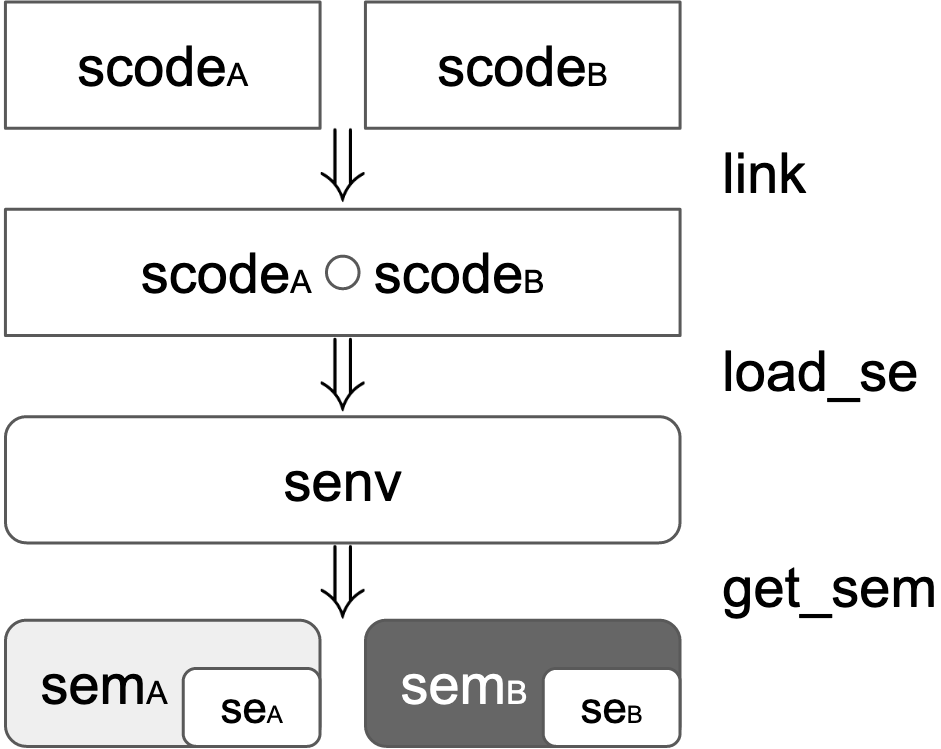
\includegraphics[width=1\linewidth]{fig-load.png}
%% \caption{Loading Process}
%% \label{fig:load}

%% \begin{minipage}{0.5\linewidth}
%% \begin{figure}
%%   \centering
%%   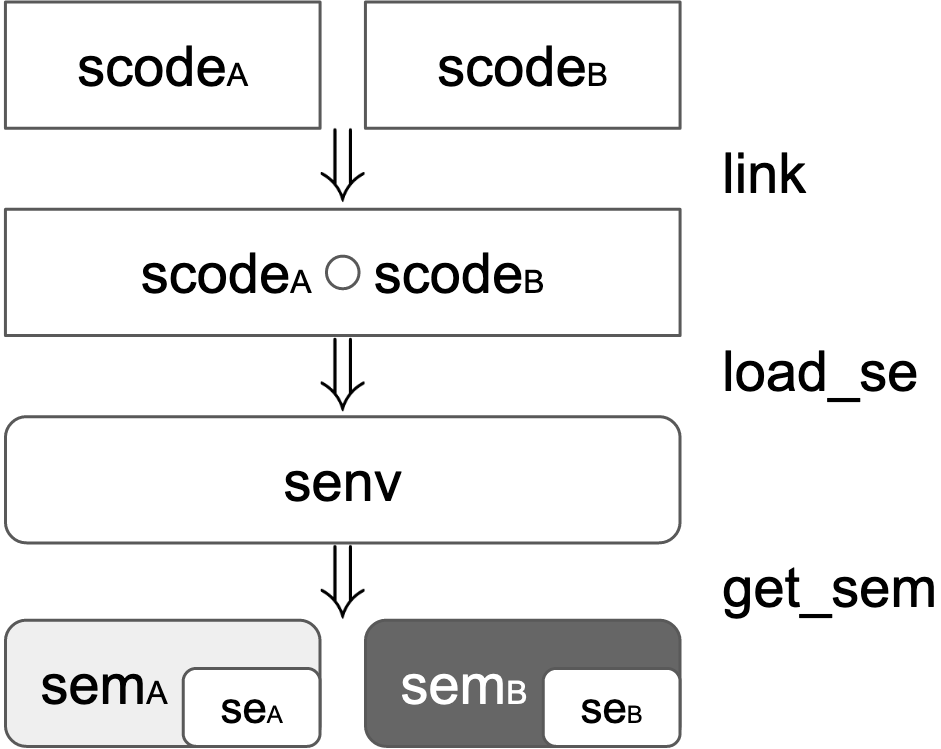
\includegraphics[width=0.25\linewidth]{fig-load.png}
%%   \caption{Loading Process}
%%   \label{fig:load}
%% \end{figure}
%% \end{minipage}

%% \begin{subfigure}{.4\linewidth}
%%   \centering
%%   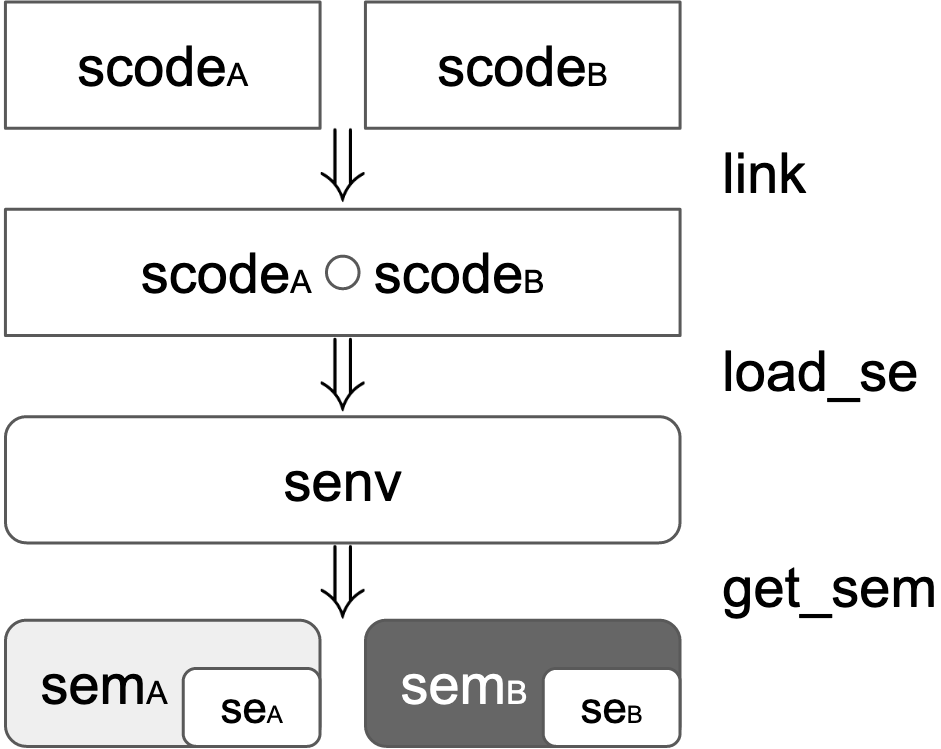
\includegraphics[width=0.25\linewidth]{fig-load.png}
%%   \caption{Loading Process}
%%   \label{fig:load}
%% \end{subfigure}

%% \youngju{lookup\_modsem is actually deterministic (loading process guarantees it)}

%% \youngju{Maybe we can use ``bar'' notation like princeton did}
\caption{Loading in Interaction Semantics}
\label{fig:full-sem}
\vspace*{-2mm}
\end{wrapfigure}



Loading the initial states of multiple modules requires an interesting
coordination of the modules, especially in the presence of module-local static variables.  In essence, we
should disallow accesses to a static variable from other modules than the defining one.  For
this, the loading of modules $M_1, \cdots, M_n$ proceeds as follows, which is illustrated for two
modules in \Cref{fig:full-sem}.

First, each module has \emph{symbol code}, which consists of symbols (\ie global variables and functions) and their
signatures (\eg{} \code{x: int}, \code{f: void(int)}).  For each $i$, let $M_i.\code{scode}$ be the
symbol code of $M_i$.  Crucially, symbol codes have the same type even if their modules are written
in different languages.

Second, since symbol codes have the same type, we can calculate the physical linking
$sc = M_1.\code{scode} \plink \cdots \plink M_n.\code{scode}$ of the symbol codes of modules.  Now
$sc$ is the symbol code for entire program consisting of all the symbols and signatures.  The
physical linking is defined in \cite{kang:scc}.

Third, we load $sc$ to get the initial memory $mem$ \newnewrevision{(by \textrm{load\_mem})}
and the program's global \emph{symbol environment}~$se$ \newnewrevision{(by \textrm{load\_se})},
which is the run-time information of symbols (\eg{} \code{x} points to
\code{0x700} and \code{f} points to \code{0x800}).  This loading process follows the original \cc{}'s.

Fourth, we initialize module semantics for each module $M_i$ with the program's global symbol
environment $se$.  In particular, we calculate $M_i$'s local environment, which contains information
of \emph{only} those symbols defined in the module.  Crucially, this prevents the other modules from
accessing the static variables of $M_i$. Note that \ccc{} does not have local environments because it does not support static variables.

Finally, the initial memory and module semantics form the initial state for interaction semantics.

%% Here, it is crucial to distinguish global and local environments for controlling accesses to
%% static variables.  Note that 

% restriction phase didn't exist in \ccc{}: instead, all the symbols were put in each module's
% symbol environment.  At that time there was no static variable, so it was fine, but now we have to
% (at least) remove other module's static variables, and we chose the most cannonical way (low
% cognitive overhead).



% Each \cc{}'s program is of type $program \; F \; V$ (static info) where F and V differs for each
% language.  F stands for function definition and V stands for info on variable definition
% (e.g. type).  Each \cc{}'s global environment (runtime info) is of type $Genv \; F \; V$.  In global
% environment, each symbol is mapped to some block in \Memory.

% communications between modules, while \ccc{} only supported C-style. Currently, Asm-style
% communication is only allowed between Asm modules (this is the same for \ccx{}.

% \youngju{FYI: bottom left of page 5 of \ccc{}'s paper explains the same thing}

% $\Skel \defeq program \; \option{sig} \; unit$ \hspace{4mm} and \hspace{4mm}
% $\Skenv \defeq Genv \; \option{sig} \; unit$ \hspace{4mm} where \hspace{4mm}
% $ \option{a} \defeq a \uplus \emptyset $.
%% \youngju{iris notation} 

% Loading process figure: square box is static info, and rounded box is runtime info. Grey ones are
% language-specific ones, and white ones are language-agnostic ones.

% Loading process should (i) give a compatible view on symbol-memory mapping, and (ii) initialize
% global variable's corresponding memory (iii) gives failure when static variable is declared in
% another module.  To this end, we use standard, off-the-shelf \cc{} linker and loader (linker is
% very slightly modified).  The linker takes uni-language modules so we first extract
% language-agnostic part of each program and to make it uni-language.  Then, we link and load it to
% get ``big'' symbol environment.  Finally, each module uses this ``big'' one to initialize its
% module semantics, resulting in ``small'' symbol environments for each one.  The ``small'' ones are
% restricted from big ones so that only symbols declared in its code are visible.  Note that, such
% restriction phase didn't exist in \ccc{}: instead, all the symbols were put in each module's
% symbol environment.  At that time there was no static variable, so it was fine, but now we have to
% (at least) remove other module's static variables, and we chose the most cannonical way (low
% cognitive overhead).

% It is not explicit in the figure, but $\texttt{load\_mem}(\texttt{A.c} \circ \texttt{B.c})$ will be
% used as an initial memory of interaction semantics.

%% \youngju{We don't need to mention (i) $\plink$ is the one introduced in \cite{TODO} and (ii) it is for single language}
% Interaction semantics is trivial, so we skip it.


% \youngju{In opensim, there are also some difference with presentation and Coq but they are
% equivalent.}

%% Note that in our overview's presentation, the language state and memory were separated.
%% But in our formalization, we chose not to: \cc{} does not separate language state and memory, and we want to reduce diff from \cc{}.
%% As a consequence, our CallData/Retdata contains memory, conveying ``current'' memory.
%% Both representations (separated or not) are equivalent.


%% \youngju{we separated memory and state in main:verification. Then, we need to separate here too}

%% \youngju{IMPORTANT: We omitted system module. However, we required $\SREL{}$ -(7) for system module, so this condition is orphaned now.}




\section{Module Semantics}
\label{sec:main-semantics:module}

%% We briefly discuss differences between the module semantics of \ccm{} presented in
%% \Cref{fig:modsem} and that of \ccc{} described in \Cref{sec:overview-semantics:background}.
%% Our module is different from that of \ccc{} on loading.

We briefly discuss the notions of module and module semantics presented in \Cref{fig:modsem}.
%
To support loading described in \Cref{sec:main-semantics:loading},
a module $M$ consists of $M\code{.scode}$, which is its symbol
code, and $M\code{.get\_sem}$, which returns a module semantics given a program's symbol environment.
The local environment \code{senv} of the module semantics should coincide with the
global environment restricted on $M\code{.scode}$.

%% The module semantics is almost the same with the presentation in the \Cref{sec:overview-semantics:background}.
%% \begin{itemize}
%% \item $\code{senv}$: A symbol environment that determines if a symbol belongs to the module semantics.
%% \item \code{init\_core}: constructs an initial machine state from the given call data, where call data is a triple representing current memory, function pointer, and its arguments. We purposely defined this operation as a predicate rather than a function in order to address nondeterminism introduced in \Cref{sec:overview-semantics:solution}.
%% \item \code{at\_external}: given a machine state, returns call data if the machine state is calling an external function, and nothing otherwise.
%% \item \code{halted}: given a machine state, returns return data (a pair representing current memory and return value) if the machine state is returning, and nothing otherwise. 
%% \item \code{after\_external}: given a machines state and return data, updates the machines state accordingly.
%% \end{itemize}

%% Few things to note here are as follows:
%% We support not only C-style but also assembly-style call and return data passing for assembly functions that does not comply with the C calling convention.
%% Assembly-style call data and return data are composed of a memory and a register file. Like \ccx{}, only assembly
%%   modules are allowed to perform assembly-style calls.

The module semantics of \ccm{} is slightly more general than that presented in \Cref{sec:overview-semantics:background}.
\begin{itemize}
\item A module semantics has a symbol environment $\code{senv}$ that determines whether a symbol belongs to the module or not.
\item \code{init\_core} is defined as a predicate rather than a function in order to allow such nondeterminism introduced in \Cref{sec:overview-semantics:solution}.
\item Module operations other than \code{corestep} (denoted here $\estep{}$) can also change the
  memory, which is needed to turn on and off the access permission of the arguments area as discussed in \Cref{sec:overview-semantics:solution}.
  %% Thanks to such flexibility, our \code{corestep} relation remains unchanged from the language steps in \cc{}.
\item Module semantics supports not only C-style but also assembly-style calling convention in the sense of \ccx{},
  where the former just passes argument and return values between the caller and callee while the latter the whole register file.
  %% which passes the whole register file information between the caller and callee instead of just argument and return values.
  %% for assembly functions that does not comply with the C calling convention.
  %% Assembly-style call and return data are composed of a memory and a register file.
  Like \ccx{}, only assembly functions are allowed to make assembly-style calls.
\end{itemize}

%% Our module semantics is different from that of \ccc{} in the following ways:
%% \begin{itemize}
%% \item A module semantics has a symbol environment $\code{senv}$ that determines if a
%%   symbol belongs to the module semantics or not.
%% \item \code{init\_core} is a predicate rather than a function to take into account nondeterminism.
%% \item Not only \code{corestep} but also all the others change memory, for the purpose of identifying
%%   core steps with the language steps in \cc{}.\footnote{Also for the purpose of identifying core
%%     steps with the language steps in \cc{}, unlike the presentation here, our Coq formalization
%%     actually does not explicitly split a machine state into a memory and a module state.}  Memory
%%   accesses introduced in interaction semantics, such as preparation for outgoing arguments area, are
%%   now performed in \eg{} \code{init\_core}.
%%   % 스텝말고 나머지도 메모리 변경.  core step = underlying step.  init\_core, ... 등에서 marshalling
%%   % 등 처리
%% \item Module semantics supports not only C-style but also assembly-style call and return value
%%   passing.  At call sites, \code{at\_external} checks if the given machine state is about to invoke
%%   an external call with a call data of type \textrm{CallData}.  A call data is either $(i)$ C-style,
%%   consisting of a memory, a function pointer, and argument values, or $(ii)$ assembly-style,
%%   consisting of a memory, a function pointer, and a register file.  On the other hand, on return,
%%   \code{after\_external} is given a return data of type \textrm{ReturnData}, and produces the next
%%   state.  A return data is also either $(i)$ C-style, consisting of a memory and a return value, or
%%   $(ii)$ assembly-style, consisting of a memory and a register file.  Like \ccx{}, only assembly
%%   modules are allowed to perform assembly-style calls.
%% \end{itemize}

\begin{figure}[t!]
\footnotesize

%% trick from: https://tex.stackexchange.com/questions/391318/make-figure-with-minipages-wider-than-text
\makebox[\linewidth]{\makebox[1.2\linewidth]{
\begin{minipage}{1.2\linewidth}
  \mytitle{module}\\
$
  \begin{stackTL}
  \begin{array}{l@{}l}
  \module \in \Module = \{ & (\texttt{scode}, \texttt{get\_sem}) \in (\Skel \times (\Skenv \rightarrow \Msem)) \; | \; \forall \skenv, \texttt{get\_sem}(\skenv).\texttt{senv} = \skenv \textbar_{\texttt{scode}}
                        \} \\
  \end{array}
  \end{stackTL}
$
\end{minipage}%
}}
\\
\makebox[\linewidth]{\makebox[1.2\linewidth]{
\begin{minipage}{1.2\linewidth}
  \mytitle{module semantics}\\
$
  \begin{stackTL}
  \begin{array}{@{}l@{}}
    \msem \in \Msem = \\
    \quad  \setof{ \myst \in \textrm{Set}, \texttt{senv} \in \Skenv, \estep{} \; \in \powset{(\Memory \times \myst) \times \Events \times (\Memory \times \myst)}, \\
    \quad\ \ \;\texttt{init\_core} \in \Args \rightarrow \powset{\Memory \times \myst}, \\
    \quad\ \ \;\texttt{at\_external} \in (\Memory \times \myst) \rightarrow \option{\Args}, \\
    \quad\ \ \;\texttt{after\_external} \in (\myst \times \Retv) \rightarrow \option{(\Memory \times \myst)}, \\
    \quad\ \ \;\texttt{halted} \in (\Memory \times \myst) \rightarrow \option{\Retv} \; | \\
    \quad\ \ \;\{ \ms \;|\; \exists e, \ms',~ \ms \estep{e} \ms' \}, \{ \ms \;|\; \exists \args, \texttt{at\_external}(\ms) = \some{\args} \},
               \{ \ms \;|\; \exists \retv, \texttt{halted}(\ms) = \some{\retv} \} \text{ disjoint}
    } \\
  \end{array}
  \\
  \begin{array}{l@{}l@{}l}
    \Args & \defeq \{ (\texttt{m}, \texttt{f}, \texttt{vs}) \in (\Memory \times \Val \times \overrightarrow{\Val}) \} & \; \uplus \;
                   \{ (\texttt{m}, \texttt{f}, \texttt{rs}) \in (\Memory \times \Val \times (\Reg \rightarrow \Val)) \} \\
    \Retv & \defeq \{ (\texttt{m}, \texttt{v}) \in (\Memory \times \Val) \} & \; \uplus \;
                   \{ (\texttt{m}, \texttt{rs}) \in (\Memory \times (\Reg \rightarrow \Val)) \} \\
    %% \args.\texttt{f} & \defeq \textbf{match} \; \args \; \textbf{with}~~
    %%                    \mathtt{|}~ \textbf{left}~ \args \Rightarrow \args.\texttt{f}~
    %%                    \mathtt{|}~ \textbf{right}~ \args \Rightarrow \args.\texttt{rs}(\textbf{PC})~
    %%                    \textbf{end} \span \\
  \end{array}
  \end{stackTL}
$
\\
\end{minipage}
}}

%% \youngju{Use [ $\defeq$ ] for [ $\module \in \Module =$ ]? If so, we should change this fig and fig-param too.}

\caption{Module and Module Semantics \vspace{5mm} \mbox{}}
\label{fig:modsem}
\end{figure}


% Like \ccc{}, we require the set of states with \code{corestep}, states \code{at\_external}, and
% \code{halted} states are disjoint.  Second, unlike \ccc{}:



% Module semantics is almost same with \ccc{}. The differences are as follows.
% (i) While their primitives (\texttt{init\_core}, \texttt{at\_external}, \texttt{after\_external}, \texttt{halted}) were function, we use Prop instead.
% For \texttt{init\_core}, it is essential --- we have introduced nondeterminisim --- but for other cases, it is rather technical (and for uniformity with \texttt{init\_core}).
% Actually, we require the other three primitives are \emph{deterministic}, so it is equivalent with function.
% (ii) Our primitives change the memory, which is for marshalling/unmarshalling. In \ccc{}' marshalling/unmarshalling was hard-coded into \texttt{corestep} relation.
% (They already re-defined \texttt{corestep} for vertical compositionality.) In contrast, we just reuse off-the-shelf step relation from \cc{}.
% (iii) We support both C-style and Asm-style communications between modules, while \ccc{} only supported C-style.

% Currently, Asm-style communication is only allowed between Asm modules (this is the same for \ccx{}.

% Symbol code ($\Skel$) and symbol environment ($\Skenv$) represents \emph{language-agnostic} part
% of \cc{}'s program/global environment (as much as one can).
%% with one mild assumption --- each function has its signature --- which is true for all \cc{} languages.
% These are used in loading interaction semantics.  We use option signature type here.  The signature
% is none for the hand-written assemblies that does not follow (C-style?) calling convention, and for
% all other cases it is some.
%% We support both C-style and asm-style for call and return.

% We will skip explaining things that are same with \ccc{}.





% \myparagraph{Asm Wrapper Semantics}

% state recognition algorithm:
% \\ (1) PC points to my function --> corestep
% \\ (2) PC does not, but it is still in genv area --> call
% \\ (3) otherwise --> return

% Mention that unfree is somewhat special/nontrivial operation: it temporarily breaks \cc{}'s axiom, but it is okay.

% \begin{itemize}
%   \item init\_core:
%     \\ (1) c.(f) points to my function, fd. %% \cdashbox{It is declared as C-style and c is actually C-style} TODOOOOOOOOOOOOOOOOOOOO
%     \\ (2) PC <-| c.f
%     \\ (3) Allocate ``dummy'' stack with (size\_arguments fd.sig). Let its block id blk.
%     \\ (4) Fill in c.vs into blk
%     \\ (5) RSP <-| (blk, 0)
%     \\ (6) Assign junk blocks of arbitrary number
%     \\ (7) RA <-| arbitrary junk pointer outside genv area
%     \\ (8) Fill in other registers with junk pointer or arbitrary non-pointer
%   \item at\_external:
%     \\ (1) PC does not points to my function, but it is still in genv area.
%     \\ (2) From $se_{big}$, find signature of corresponding function.
%     \\ (3) Read list val from my arguments area, (vs).
%     \\ (4) Free my arguments area
%     \\ (5) c <-| (PC, current mem, vs)
%   \item after\_external:
%     \\ (1) $PC_{current}$ <-| $RA_{before}$
%     \\ (2) Make caller-save registers undef
%     \\ (3) RAX (return register) <-| r.v
%     \\ (4) Unfree my arguments area, and fill it with undef
%   \item final\_frame:
%     \\ (1) PC does not points to my function, and it is not in genv area
%     \\ (2) Check PC is same with initial RA
%     \\ (3) Do callee-save checking with inital registers.
%     \\ (4) Free my ``dummy stack''.
%     \\ (5) r <-| (r, current mem)
% \end{itemize}

% Mention we also support asm-style passing.
% As mentioned before, asm-style passing is only allowed between assembly modules.
% We just pass (both in call and return) current register set and memory directly.
% The only one exception is \textbf{RA} register: it exactly follows C-style convention, in order to use ``state recognition algorithm'' above.
% \textbf{RA} is \cc{}-specific pseudo register so we can do what we want.




%%% Local Variables:
%%% mode: latex
%%% TeX-master: "main"
%%% End:

